\documentclass[12pt, a4paper]{article}
\usepackage[utf8]{inputenc}
\usepackage[english]{babel}
\usepackage{amsmath}
\usepackage{amsfonts}
\usepackage{amssymb}
\usepackage{csquotes}
\usepackage{mathtools}
\usepackage{graphicx}
\usepackage{geometry}
\usepackage{setspace}
\usepackage{longtable}
\usepackage{float}
\usepackage{comment}
\usepackage{listings}
\usepackage{fancyhdr}
\usepackage{blindtext}
\usepackage[colorlinks=true, allcolors=blue]{hyperref}

\usepackage[style=authoryear]{biblatex}
\addbibresource{Bibliography.bib}

\geometry{top = 2.5cm, bottom = 2.5cm, left= 3cm, right= 3cm}

\fancypagestyle{mystyle}
{
    \rhead{Experiment 5}
    \lfoot{Lee Farrugia}
    \cfoot{}
    \rfoot{Page \thepage}
    \renewcommand{\headrulewidth}{0pt}
    \renewcommand{\footrulewidth}{0.5pt}
}

\fancypagestyle{titlepagestyle}
{
    \fancyhf{}
    \lfoot{Lee Farrugia}
    \cfoot{}
    \rfoot{Page \thepage}
    \renewcommand{\headrulewidth}{0pt}
    \renewcommand{\footrulewidth}{0.5pt}
}

\title{The Balmer Series}
\author{Lee Farrugia \\ Experiment 5 \\ Group 1A}

\date{25$^{\text{th}}$ March 2022}

\begin{document}

\maketitle
\thispagestyle{titlepagestyle}
\pagestyle{mystyle}

\section*{Aim}
The aim of this experiment was to determine the value of Rydberg's constant from the radiation of Hydrogen.

\section*{Diagram}
\begin{figure}[H]
    \centering
    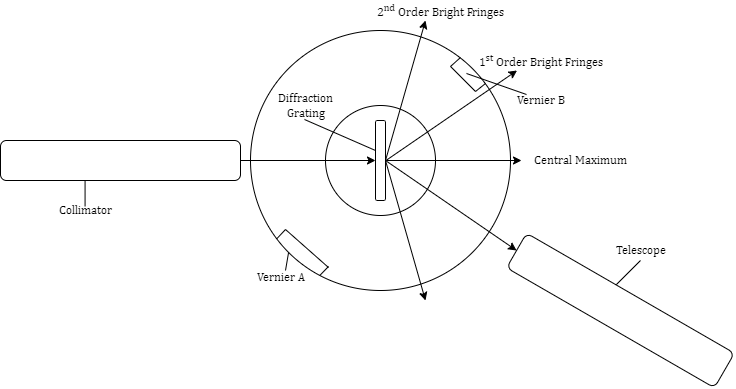
\includegraphics[width = \textwidth]{Experiment 5.png}
    \caption{Apparatus Set up}
    \label{fig:set up}
\end{figure}

\section*{List of Apparatus}
Spectrometer, diffraction grating, hydrogen lamp, power supply, lens and lamp with red covering.

\section*{Language and Packages}
Python 3.9.7, Matplotlib.pyplot, Pandas, Numpy

\section*{Procedure}
\begin{enumerate}
    \item The spectrometer was taken outside in order to be focused on the Chemistry building. A tutor was asked to confirm that the spectrometer was properly focused.
    \item The crosshair of the telescope was placed on the centre of the beam of light from the hydrogen lamp. The angle of the telescope was read from the vernier and noted. 90$^{\circ}$ was then added to the angle and the telescope was locked.
    \item With the telescope perpendicular to the collimator, a mirror was used to see the beam from the lamp. The angle of the mirror was noted and a further 45$^{\circ}$ was added to this in order to obtain 90$^{\circ}$, and thus making it parallel to the collimator.
    \item The diffraction grating was placed into the spectrometer, instead of the mirror. The telescope crosshair was again placed on the centre of the beam from the hydrogen lamp.
    \item The telescope was moved to one side of the central beam until the violet spectral line was found. The crosshair of the telescope was placed at the centre of the spectral line and the angle of the telescope was read from both the verniers.
    \item This was repeated for all the 4 different colours visible, i.e. violet, blue, cyan and red.
    \item The telescope was then moved to the opposite side of the central beam and the same procedure for finding the angles was done for all 4 colours. 
    \item All the angles obtained were noted in the table below.
\end{enumerate}

\section*{Precautions}
\begin{itemize}
    \item[-] The room was as dark as possible.
    \item[-] The opening of the lamp was shielded as much as possible.
    \item[-] The spectral lamp was turned on from before hand, in order to allow it to reach its maximum temperature.
    \item[-] Time was allowed to pass before viewing the fringes, as to allow the eye to adjust to the darkness.
    \item[-] A lamp was covered with red plastic as to limit the amount of light when reading from the verniers. 
\end{itemize}

\section*{Sources of Error}
\begin{itemize}
    \item[-] The diffraction grated may have had manufacturing errors, making certain end fringes hard to see.
    \item[-] Over time with repeated use the lamp may have become dimmer.
    \item[-] The spectrometer although calibrated at a distance, it was not calibrated at infinity.
    \item[-] Even though the room was as dark as possible some light had entered. 
    \item[-] The lenses of the telescope grating might not have been clean.
    \item[-] The diffraction grating might not have been clean.
\end{itemize}

\section*{Data and Graphs}
\renewcommand*{\arraystretch}{1.2}
\begin{longtable}{|c|c|c|c|c|}
\hline \textit{Colour} & $A$/$ ^{\circ}$ & $A'$/$^{\circ}$ & $B$/$^{\circ}$ & $B'$/$^{\circ}$\\
\hline  & \textpm $\frac{1}{120}$ & \textpm $\frac{1}{120}$ & \textpm $\frac{1}{120}$ &\textpm $\frac{1}{120}$\\ \hline
\endfirsthead

\hline \textit{Colour} & $A$/$ ^{\circ}$ & $A'$/$^{\circ}$ & $B$/$^{\circ}$ & $B'$/$^{\circ}$\\
\hline  & \textpm $\frac{1}{120}$ & \textpm $\frac{1}{120}$ & \textpm $\frac{1}{120}$ &\textpm $\frac{1}{120}$\\ \hline
\endhead

violet & 69.25 & 101.44 & 249.13 & 281.42 \\ \hline
blue   & 69.08 & 101.74 & 249.00 & 281.85 \\ \hline
cyan   & 68.11 & 102.58 & 248.15 & 282.42 \\ \hline
red    & 63.01 & 107.26 & 242.85 & 287.19 \\ \hline
\caption{Data of colour of fringes and their corresponding angles}
\label{Tab:Table 1}\\
\end{longtable}

\begin{figure}
    \centering
    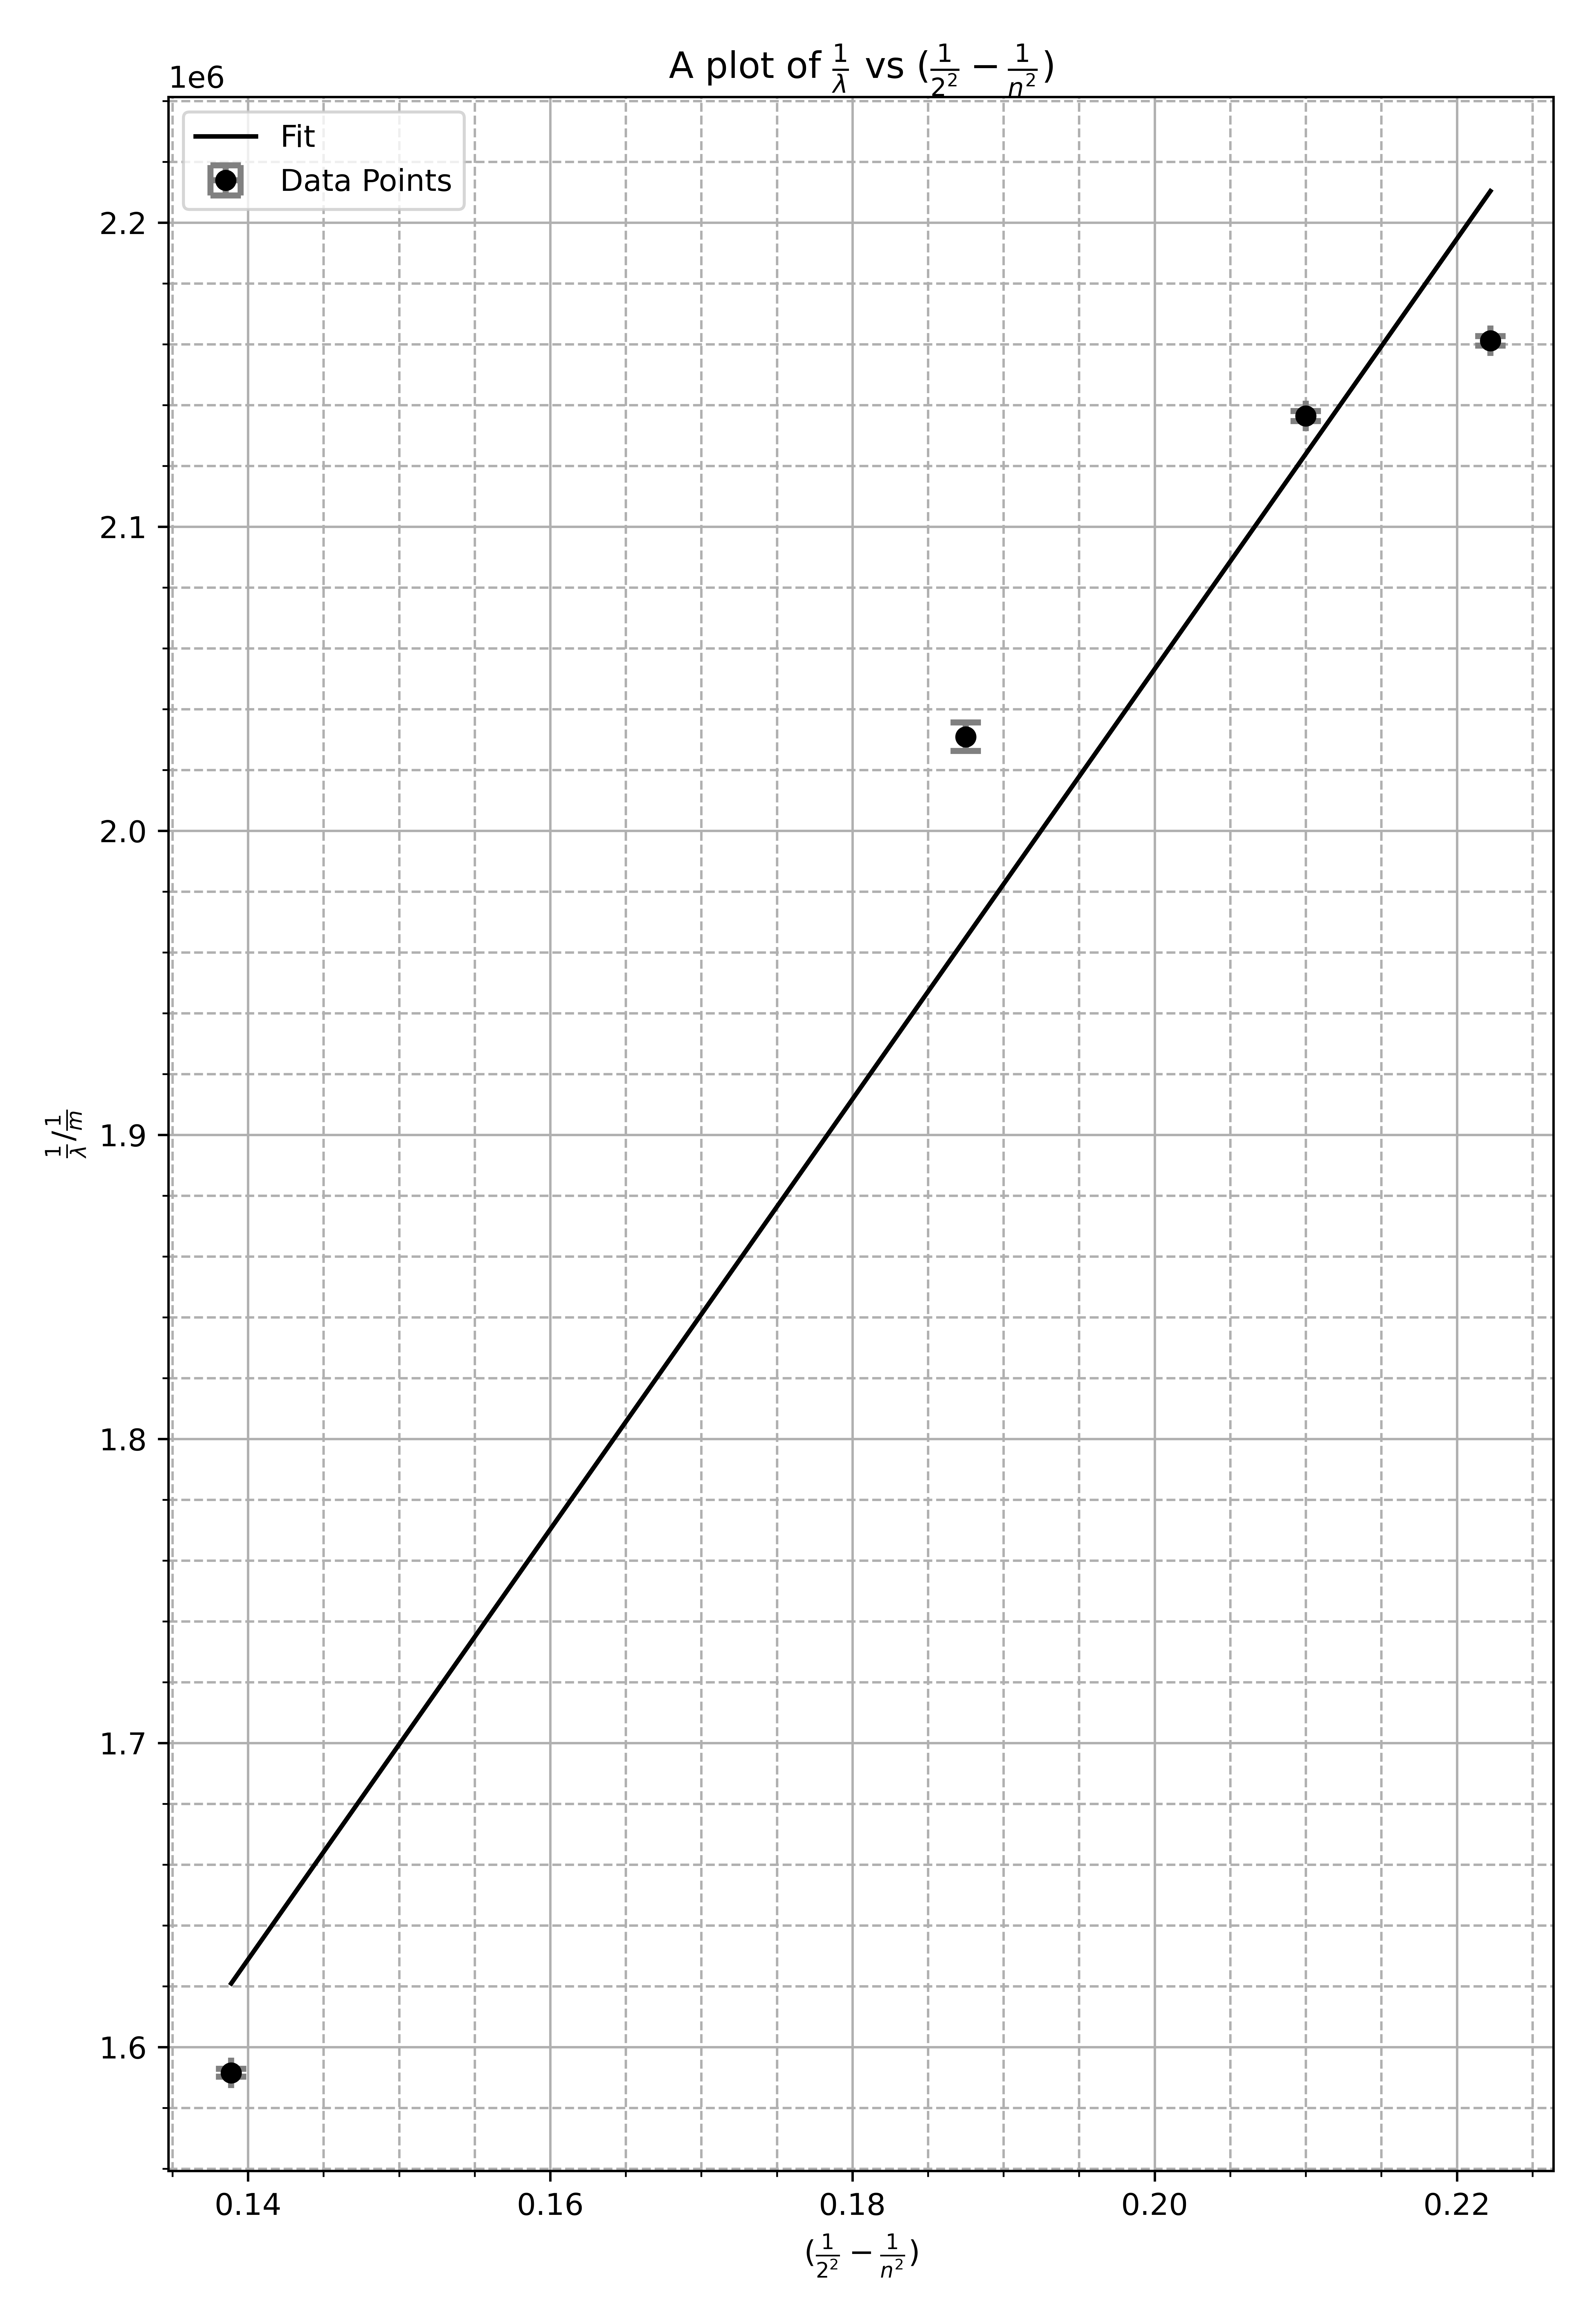
\includegraphics[width = \textwidth]{l vs x.png}
    \caption{$\frac{1}{wavelength}$ vs $(\frac{1}{2^2}-\frac{1}{n^2})$}
    \label{fig:graph}
\end{figure}

\section*{Calculations}
The data gathered during the experiment was imported into the program by using the following line of code:
\begin{lstlisting}
    data = pd.read_excel(`Experiment 5.xlsx').
\end{lstlisting}
The angles of each bright fringe was defined by the following lines of codes:
\begin{lstlisting}
    A = np.asarray(data[`A'])
    Ap = np.asarray(data[`'Ap'])
    B = np.asarray(data[`B'])
    Bp = np.asarray(data[`Bp']),
\end{lstlisting}
where $A$ is the angle read from the vernier on on side of the vernier on on side of the central beam and $Ap$ id the angle read from the vernier on the other side of the central beam, the same follows for $B$ and $Bp$. The diffraction grating number of lines per meter and the $n$ value for each colour were defined by the following lines of code:
\begin{lstlisting}
    d = 1/600000
    n = np.array([6,5,4,3]).
\end{lstlisting}
In order to obtain the angle for each bright fringe the following equation were used:
\begin{align*}
    \theta_A &= \left|\left(\frac{A'-A}{2}\right)\right|\,,\\
    \theta_B &= \left|\left(\frac{B'-B}{2}\right)\right|\,,\\
    \theta &= \left(\frac{\theta_A + \theta_B}{2}\right)\,,
\end{align*}
where $\theta_A$ is the overall angle from vernier A, $\theta_B$ is the overall angle from vernier B and $\theta$ is the average angle for each colour. The angle obtained was then used in order to obtain the wavelength for each colour by using the following equation:
\begin{equation*}
    d\sin(\theta)=n'\lambda\,,
\end{equation*}
where $d$ is the spacing between the lines of the diffraction grating, $n'$ is the order of the observed fringes which in the case was only the first order, and $\lambda$ is the wavelength. The equation was rearranged to:
\begin{equation*}
    \lambda = d\sin(\theta)\,.
\end{equation*}
In order to obtain the Rydberg's constant the following equation which links the wavelength with the $m$ and $n$ values of the bright fringes:
\begin{equation*}
    \frac{1}{\lambda}=R_H\left(\frac{1}{m^2}-\frac{1}{n^2}\right)\,,
\end{equation*}
this equation was compared to the straight line equation of $y=\text{m}x+\text{c}$, where $y$ would be equal to $\frac{1}{\lambda}$ and $x$ would be equal to $\left(\frac{1}{m^2}-\frac{1}{n^2}\right)$. The $m$ used in this formula was set 2 thus resulting that $m^2=4$. The gradient m from the straight line equation would be equal to $R_H$. This was found to be $7.07\times10^6\text{ m}^{-1}$. In order to obtain the error of the gradient, the data collected was used to find the coefficients of the best straight line possible, and then plotted. The co-variance matrix produced from finding the best straight line was used to find the error by square rooting the correct position. All of this was done by the following lines of code:
\begin{lstlisting}
    coeffs, cov = np.polyfit(X, Y, deg=1, cov=True)
    poly_funct= np.poly1d(coeffs)
    trendline = poly_funct(X)
    error = np.sqrt(cov[0][0]).
\end{lstlisting}
This resulted in the Rydberg's constant being equal to $7.07\times10^6 \pm 9.82\times10^5 \text{ m}^{-1}$. In order to find the error bars for each value obtained, it was first noted that n has no error as it was given, while in the case of $\lambda$ the following equations were used:
\begin{align*}
    \Delta\theta_A &= \sqrt{(\theta_A \times \Delta A)^2 + (\theta_{A'} \times \Delta A')^2}\\
    \Delta\theta_B &= \sqrt{(\theta_B \times \Delta B)^2 + (\theta_{B'} \times \Delta B')^2}\\
    \Delta\theta &= \sqrt{(\theta \times \Delta\theta_A)^2 + (\theta \times \Delta\theta_B)^2}\\
    \Delta\lambda &= \left(\frac{\partial}{\partial\theta}d\sin{\theta}\right) \times \Delta\theta\\
    &= d\cos{\theta}\times \Delta\theta\,,
\end{align*}
this was done with the following lines of code:
\begin{lstlisting}
    dt = np.sqrt((theta1*dA**2) + (theta2*dB**2))
    dtf = np.sqrt((theta*dt**2) + (theta*dt**2))
    dw = (d*(np.cos(theta))*dtf)
    dl =(1/np.sqrt(np.abs(dw))).
\end{lstlisting}
The accuracy and precision of the obtained values were found using the following equations:
\begin{align*}
    \text{Accuracy} &= \frac{\text{Experimental Value}}{\text{Actual Value}} \times 100\% \\
    \smallskip
    \text{Precision}&=\frac{\text{Combined Error}}{\text{Experimental Value}} \times 100\% \,,
\end{align*}
this was done through the following lines of code:
\begin{lstlisting}
    accuracy = (coeffs[0]/1.097e7)*100
    precision = (error/coeffs[0])*100,
\end{lstlisting}
the accuracy was found to be 64.48\% and the precision was 13.88\%.

\section*{Discussion}
Rydberg's constant was found to be $7.07\times10^6 \pm 9.82\times10^5 \text{ m}^{-1}$ while the real value is quoted to be $1.097\times10^7 \text{ m}^{-1}$ \parencite{muncaster}. This resulted that the accuracy of the value obtained from the experiment was 64.48\%, while it had a precision of 13.88\%. As the accuracy was below 90\% and precision was higher than 10\%, this means that the obtained value is not as accurate as one would hope and the precision although close to the cut off point was still too high. This could have been due to the fact that the diffraction grating used had manufacturer errors and also due to the fact that the hydrogen lamp used might have dimmed down due to the repeated use over the years.

\medskip
\noindent
In his experiment Compton found that the wavelength of scattered radiation is larger than the incident radiation, which in classical theory this does not hold. Classical theory states that both the incident and scattered radiation should have the same wavelength \parencite{muncaster}. As classically it is assumed that the energy of the incident X-ray radiation is too large to be absorbed thus the electromagnetic wave produced from the oscillating electron would have the same wavelength \parencite{Quantum}. It was also noted that the intensity of the incident radiation and the scattered radiation are also not the same. From this Compton noticed that the wavelength each time increased by $\Delta\lambda$, which he called the wavelength shift and it was dependent on the scatter angle rather than the intensity of the incident radiation. The only which Compton could explain his results was with treating the incident radiation as if it was made up out of particles, which on coming in contact with the free electrons would collide with them elastically \parencite{Quantum}. This correlates with the Quantum reasoning that radiation can behave as both a particle and a wave.

\section*{References}
\printbibliography[heading=none]

\section*{Appendix}
\lstset{language=Python,
    showstringspaces=false,
    showtabs=false}
\begin{lstlisting}
import numpy as np
import pandas as pd
import matplotlib.pyplot as plt

# importing data
data = pd.read_excel(`Experiment 5.xlsx')
# defining variables and constants
A = np.asarray(data[`A'])
Ap = np.asarray(data[`'Ap'])
B = np.asarray(data[`B'])
Bp = np.asarray(data[`Bp'])
d = 1/600000
n = np.array([6,5,4,3])
dA = 1/120
dB = 1/120

# finding the angles from the repeated readings
theta1 = np.absolute(A-Ap)/2
theta2 = np.absolute(B-Bp)/2
# finding the average of the angles
theta = (theta1 + theta2)/2
# finding the error for each value
dt = np.sqrt((theta1*dA**2) + (theta2*dB**2))
dtf = np.sqrt((theta*dt**2) + (theta*dt**2))
dw = (d*(np.cos(theta))*dtf)
dl =(1/np.sqrt(np.abs(dw)))

# finding the wavelength
wavelength = d*np.sin(np.deg2rad(theta))

# defining plotting arrays
Y = 1/wavelength
X = ((1/2**2)-1/(n**2))

# determining the line of best fit
coeffs, cov = np.polyfit(X, Y, deg=1, cov=True)
poly_funct= np.poly1d(coeffs)
trendline = poly_funct(X)
# defining the error of Rydberg's constant
error = np.sqrt(cov[0][0])
print(f``Rydberg's constant is {coeffs[0]:.2e}
         with an error of {error:.2e}")

# finding the accuracy and the precision
accuracy = (coeffs[0]/1.097e7)*100
precision = (error/coeffs[0])*100
print(f`The accuracy was found to be {accuracy:.2f}%
        and a precision of {precision:.2f}%')

# defining the size of the figure
f = plt.figure(figsize=(7.3, 10.7))

# defining the plot line, points, error bars
plt.errorbar(X, Y, xerr=0, yerr=dl, fmt=`o', 
             color=`k', elinewidth=2, capthick=2, capsize=5,
             ecolor=`grey', label=`Data Points')
plt.plot(X, trendline, color=`k', label=`Fit')
# defining axis labels, title, grid, legend and showing plot
plt.minorticks_on()
plt.grid(b=True, which=`major', linestyle=`-')
plt.grid(b=True, which=`minor', linestyle=`--')
plt.xlabel(r`$(\frac{1}{2^2}-\frac{1}{n^2})$')
plt.ylabel(r`$\frac{1}{\lambda}$/$\frac{1}{m}$')
plt.title(r`A plot of $\frac{1}{\lambda}$ 
            vs $(\frac{1}{2^2}-\frac{1}{n^2})$')
plt.legend()
# removing wasted space from graph boundaries
plt.tight_layout()
# saving plot
plt.savefig(`l vs x.png', dpi=800)
plt.show()
\end{lstlisting}

\end{document}
